\chapter{Problem Statement} \label{chap:chap3}

In this chapter the problem will be described and justified, using references from the bibliographic study presented in Chapter~\ref{chap:sota}.

\section{Problem Description}

Currently, FEUP's computing infrastructures are only accessed by those who have the technical knowledge to interact with the system. These people are technicians whose area of expertise encompasses outsourcing computing resources to perform computing jobs. 

If someone from an area unrelated to the computing system wants to perform any operation in it, that someone must contact the said technicians and waste valuable time for both parties cutting through red tape.

Having this in mind, CICA has started developing a project that reduces the ammount of knowledge necessary to perform the said computing operations.

This document focuses only on the front-end of the project, the back-end having already been developed by former MIEIC student Nuno Cardoso as part of his Master Thesis. CICA's project is described in greater detail in the following section.

\section{The project} \label{sec:project}


The project aims at simplifying the whole process and to make FEUP's computing infrastructures more accessible to the academic community, without the users having to spend time learning about the technologies and how the system actually works.

In order to better understand the full scope of the issue, Figure~\ref{fig:big_picture} shows the full system as it should function, through the means of an hypotetic and yet plausible use case scenario:

\begin{figure}[t]
  \begin{center}
    \leavevmode
    \fbox{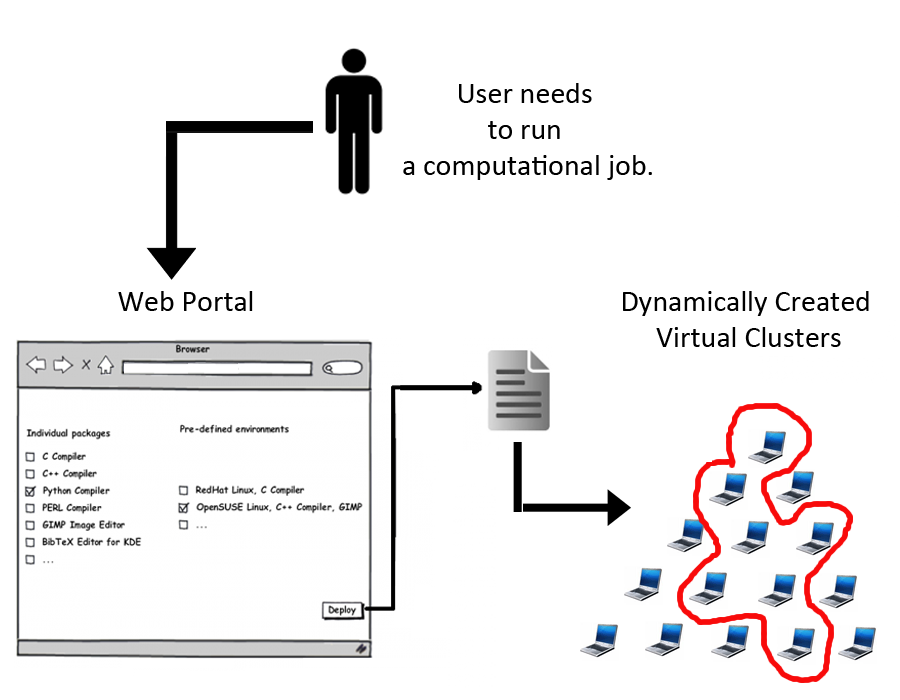
\includegraphics[width=\linewidth]{big_picture.png}}
    \caption{CICA's full computing project.}
    \label{fig:big_picture}
  \end{center}
\end{figure}

Firstly, a researcher of a specific field of study wants to conduct a more complex operation that involves greater computing efforts than his/her home and work computer. As such, the researcher proceeds to enter the designed system through a web page where he/she can:

\begin{itemize}
	\item Chose a suitable work environment for her computational needs according to a set of predefined parameters;
	\item Create his/her own work environment according to the specifications he/she provides the system with.
\end{itemize}

The system will then automatically create a virtual environment (image containing all the information needed), which will be passed onto the back-end of the project where a virtual cluster will be created according to that virtual environment.
Finally a username and password combination should be returned so that the researcher can enter the created environment and perform his/her operations. 

\section{The solution}\label{sec:solution}

One of the main objectives of this dissertation is the integration of an \textit{OpenStack} --- presented in Chapter~\ref{chap:sota} --- deployment environment as it should simplify the cloud creation and management.

One thing that was missing in the cloud computing scene, was a cloud management layer. A cloud operating system that added automation and control at scale. That is where \textit{OpenStack} comes into play. As mentioned in Chapter~\ref{chap:sota}, it is built by a world wide community of developers, something that made it a good choice to investigate, as the open source culture is something always worthy of enriching.~\cite{https://github.com/dellcloudedge/crowbar/wiki/OpenStack-Essex-Deploy-Day}

There is one thing one must keep in mind: as it was described in Chapter~\ref{chap:sota}, \textit{OpenStack} is not the only solution available. \textit{OpenNebula} was also available, but \textit{OpenStack} is a more recent project and \textit{OpenNebula} is already up and running at FEUP. 

Furthermore, \textit{OpenStack} is written in \textit{Python} whereas \textit{OpenNebula} is written in \textit{Ruby on Rails}. There was already a previous experience with \textit{Rube on Rails} (a not so favourable one) and since there was a desire for new challenges and learning new programming languages, \textit{OpenStack} was chosen. This would also allow to contribute to FEUP's knowledge on this new technology.

Rodrigo Benzaquen, director of site operations and infrastructure at MercadoLibre, a Latin America e-commerce market leader which chose to use \textit{OpenStack} as their cloud solution, stated the following:

\begin{quote}
 ``Before this [\textit{OpenStack}'s deployment], we would have had someone physically deploy the server which would take a day or longer. With \textit{OpenStack}, we don't have to do that; our developers are now able to create and manage their servers.''\cite{openstack_userstories}
\end{quote}

which came directly into the objective of this dissertation, easing the cloud creation and management process.

\subsection{Connecting the dots}\label{subsec:architecture}

As mentioned in Chapter~\ref{chap:sota}, section~\ref{subsec:openstack}, \textit{OpenStack} is designed to deliver a massively scalable cloud operating system, each of the components being designed to work together in order to prodive complete IaaS. This integration is facilitated through pulic APIs that each service offers, being available to the cloud's end users.~\cite{http://ken.pepple.info/openstack/2012/02/21/revisit-openstack-architecture-diablo/}. 

Expanding the diagram shown in Figure~\ref{fig:openstack_sw_diag}, the relationships between the services are shown in Figure~\ref{fig:openstack_services}:

\begin{figure}[H]
  \begin{center}
    \leavevmode
    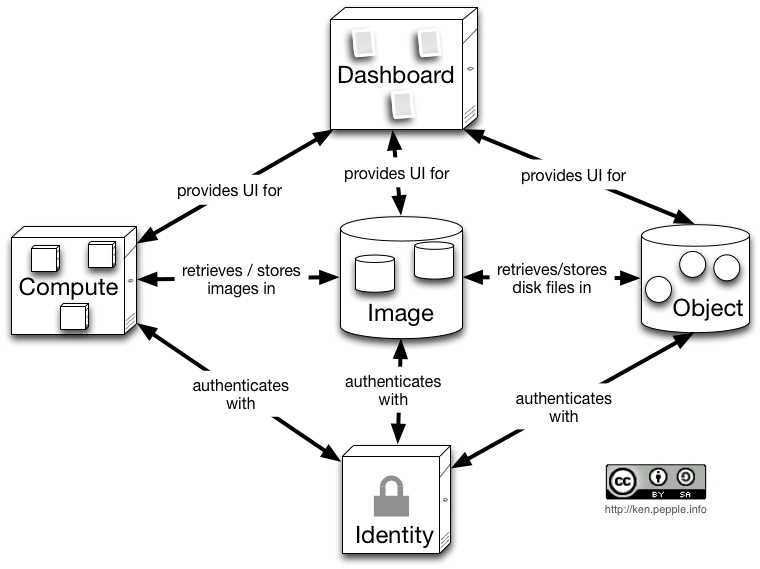
\includegraphics[scale=0.5]{nova-concept-int-essex}
    \caption{Relationships between the different \textit{OpenStack} services\cite{http://ken.pepple.info/openstack/2012/02/21/revisit-openstack-architecture-diablo/}.}
    \label{fig:openstack_services}
  \end{center}
\end{figure}

The solution proposed for this project links the \textit{OpenStack} Dashboard --- \textit{Horizon} --- with the designed \textit{Web application} developed in \textit{Python} and \textit{Django}, as shown in Figure~\ref{fig:architecture}.







The issue and the approach taken to solve it.
Este capítulo deve começar por fazer uma apresentação detalhada do
problema a resolver\footnote{Na introdução a apresentação do
  problema foi breve.} podendo mesmo, caso se justifique,
constituir-se um capítulo com essa finalidade.

Deve depois dedicar-se à apresentação da solução sem detalhes de
implementação. 
Dependendo do trabalho, pode ser uma descrição mais teórica, mais
``arquitectural'', etc.

\section{Resumo e Conclusões}

Resumir e apresentar as conclusões que se podem tirar no fim deste
capítulo.
